Assume that our current released version of software product is \texttt{v1.0.0}
and there is a critical bug appears.
In order to release a hotfix the following set of steps to be performed
\begin{enumerate}
    \item Hotfix to be assigned to a software engineer.
    \item Software engineer creates a new branch \texttt{hotfix/*} from the latest \texttt{Release/v*} branch.
    \item Software engineer fixes the bug in the \texttt{hotfix/*} branch.
    \item Software engineer creates a pull request \texttt{hotfix/* -> release/v*}.
    \item The pull request \texttt{hotfix/* -> release/v*} is reviewed by team and merged.
    \item Release engineer creates a new tag \texttt{v1.0.1} from the latest \texttt{release/v*} branch.
    \item Hotfix deployment process is started after new tag is pushed.
    \item Hotfix is deployed to production.
    \item Release engineer creates a pull request \texttt{release/v* -> master} that contains the hotfix.
    \item The pull request \texttt{release/v* -> master} is reviewed by team and merged.
\end{enumerate}
\begin{figure}[H]
    \centering
    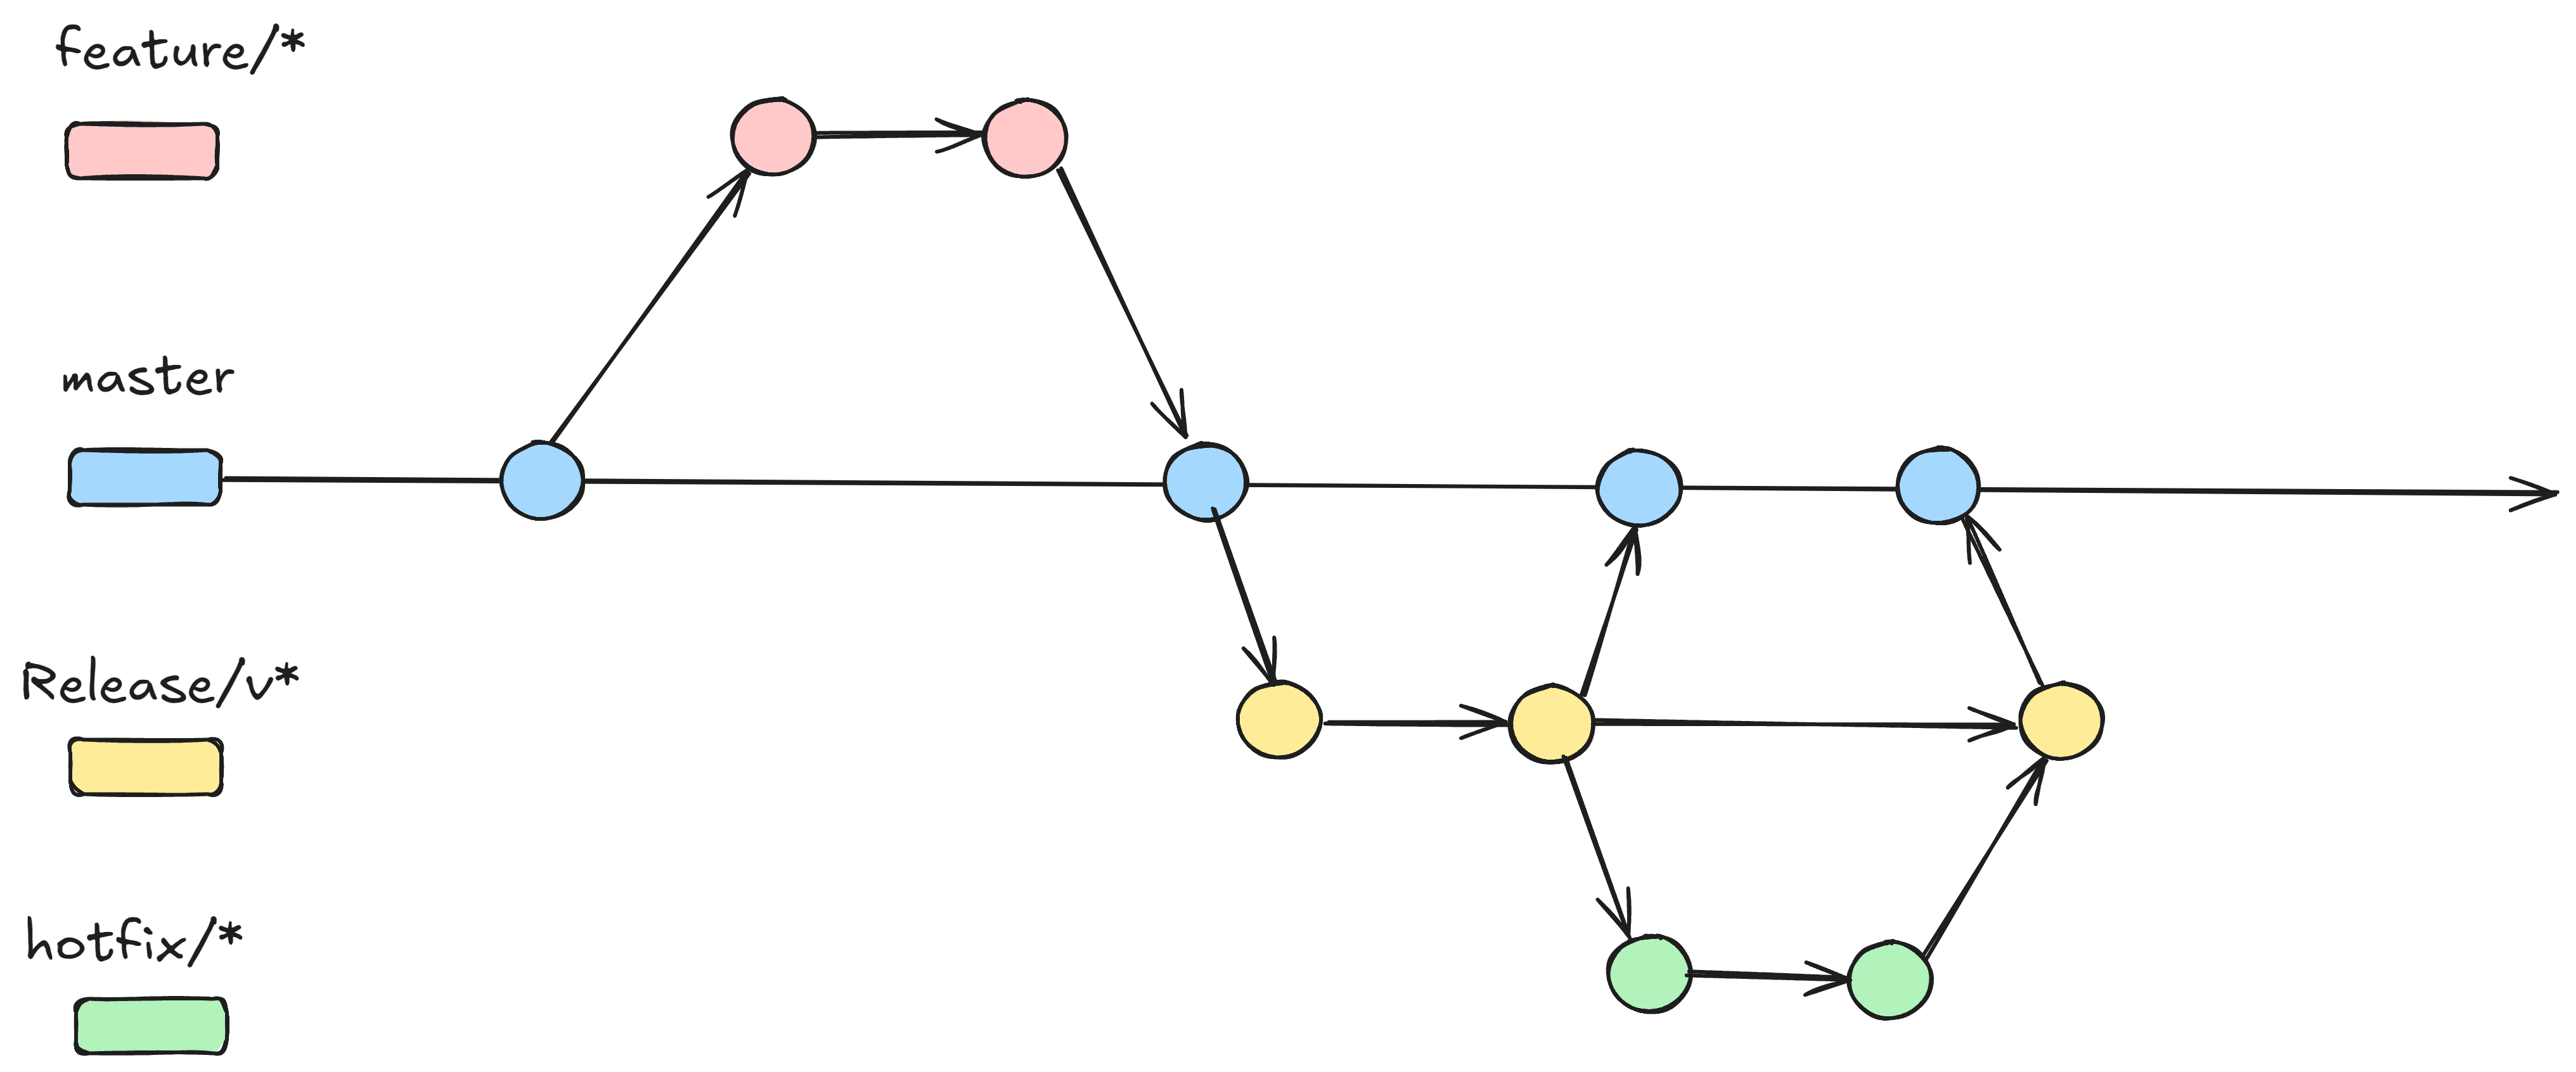
\includegraphics[width=1\textwidth]{img/HotFix_Strategy}
    ~\caption{Hotfix diagram.}\label{fig:hotfix-diagram}
\end{figure}

